\documentclass[a4paper,12pt]{article}
\usepackage[utf8]{vietnam}
\usepackage{graphicx}
\usepackage{geometry}
\usepackage{tikz}
\usetikzlibrary{calc}
\usepackage{xcolor}
\usepackage{enumitem}
\usepackage{titlesec}
\usepackage{helvet}
\usepackage{mdframed}
\usepackage{verbatim}
\renewcommand{\familydefault}{\sfdefault}
\geometry{margin=2.5cm}

\begin{document}
\fontsize{14pt}{16pt}\selectfont
\begin{titlepage}
\begin{center}
 
\begin{tikzpicture}[remember picture, overlay]
  \draw[line width=0.5pt] 
    ($ (current page.north west) + (1.5cm,-1.5cm) $) rectangle 
    ($ (current page.south east) + (-1.5cm,1.5cm) $);
\end{tikzpicture}

\vspace*{0.5cm}
\textbf{POSTS AND TELECOMMUNICATIONS INSTITUTE OF TECHNOLOGY}\\[0.2cm]
\textbf{FACULTY OF INFORMATION TECHNOLOGY 1}\\[1.5cm]
\begin{figure}[h]
    \centering
    \includegraphics[width=0.5\textwidth]{ptit-logo.png}
\end{figure}
\textbf{\Large PYTHON PROGRAMMING}\\[0.5cm]
\textbf{ASSIGNMENT 1}\\[0.5cm]
\textbf{\LARGE FOOTBALL DATA ANALYSIS}\\[3cm]



{\Large
\begin{center}
\begin{tabular}{ll}
\textbf{Instructor} & Kim Ngoc Bach \\
\textbf{Student} & Nguyen Thi Nhung \\
\textbf{Student ID} & B23DCVT322 \\
\textbf{Class ID} & D23CQCE04-B \\
\end{tabular}
\end{center}
}

\vfill
\textit{Hanoi}

\end{center}
\end{titlepage}

\newpage
%_______Mục lục________
\begin{center}
    \textcolor{blue}{\textbf{\Large TABLE OF CONTENTS}}
\end{center}

\begin{enumerate}[label=\textbf{\arabic*.}, leftmargin=1.5cm]
    \item \textbf{INTRODUCTION}
    \item \textbf{COLLECTING STATISTICAL DATA OF PREMIER LEAGUE FOOTBALL PLAYERS}
    \item \textbf{DATA ANALYSIS}
    \begin{enumerate}[label=\arabic{enumi}.\arabic*.]
        \item Identity the Top 3 players with the Highest and lowest for each statistic
        \item  Find the median, calculate the mean and the standard deviation
        \item Plot histogram showing the distribution of each statistic for all players.
        \item Identifying the Best-Performing Team
    \end{enumerate}
    \item \textbf{PLOT 2D VISUALIZATION OF STATISTICAL DATA}
    \item \textbf{PLAYER VALUE ESTIMATION}
    \begin{enumerate}
    [label=\arabic{enumi}.\arabic*.]    \item Collect valuable player transfer data (2024-2025)
    \end{enumerate}
    \item \textbf{CONCLUSION}
\end{enumerate}

\newpage
%_______Giới thiệu________
\section*{\textcolor{blue}{\Large 1. Introduction}}

\setlength{\parindent}{0pt}  
\setlength{\parskip}{1em} 
In recent years, data analysis has become a crucial component of professional sports, particularly football. Clubs, analysts, and fans increasingly rely on statistical data to evaluate player performance, optimize match strategies, and support financial decisions such as player transfers.

This project aims to apply the Python programming language to collect, process, and analyze player statistics from the 2024–2025 English Premier League season.

The first objective is to develop an automated system that retrieves a wide range of performance metrics from public sources, specifically fbref.com — a reputable football statistics website. The data includes indicators such as playing time, goals, assists, expected goals (xG), defensive actions, passing statistics, and more. Only players with over 90 minutes of playtime are included in the dataset, which is stored in a file named results.csv.

The second objective is to conduct statistical analysis to identify top-performing players, compute summary statistics such as mean, median, and standard deviation, and visualize data distributions through histograms. The project also aims to determine which group of players performs best based on aggregated performance metrics.

In addition, clustering techniques using the K-Means algorithm combined with Principal Component Analysis (PCA) are applied to reduce dimensionality and group players with similar performance characteristics. The clustering results are displayed in a 2D plot for ease of interpretation and analysis.

Finally, the project incorporates player market value data from footballtransfers.com and applies a machine learning approach — specifically Random Forest Regression — to estimate market value based on in-game performance statistics. This process involves data preprocessing, feature selection, model training, and evaluation using metrics such as Mean Squared Error (MSE).

Through this project, the author not only strengthens practical skills in Python-based data science but also gains deeper insights into how statistical methods and machine learning algorithms can be applied in real-world sports analytics, laying a solid foundation for future research and broader applications.
\newpage
%_______Bài 1________
\section*{\textcolor{blue}{\Large 2. Collecting statistical data of premier league football players}}
The data is collected from the following web pages of the FBRef website:
\begin{itemize}
    \item \texttt{stats\_standard}: General player statistics
    \item \texttt{stats\_keeper}: Goalkeeper statistics
    \item \texttt{stats\_keeper\_adv}:
    Advanced Goalkeeper Stats
    \item \texttt{stats\_shooting}: Shooting statistics
    \item \texttt{stats\_passing}: Passing statistics
    \item \texttt{stats\_passing\_types}: Passing Types Statistics
    \item \texttt{stats\_gca}: Goal Creation Actions (GCA) statistics
    \item \texttt{stats\_defense}: Defensive statistics
    \item \texttt{stats\_possession}: Possession statistics
    \item \texttt{stats\_misc}: Miscellaneous statistics
\end{itemize}

The URLS for these pages are stored in a dictionary (url\_dict) for easy access.

\titleformat{\section}
  {\bfseries\Large}
  {\thesection.}{1em}{}

\setlist[itemize]{noitemsep, topsep=0pt}

\textbf{a) Web Scraping} \\
The script uses Selenium to automate a headless Chrome browser and scrape HTML tables. The implementation corresponds to the following steps:
\begin{itemize}
    \item Send an HTTP request using Selenium: The \texttt{init\_driver()} function launches a headless Chrome browser. The \texttt{get(url)} method navigates to the target URL.
    \item Parse the returned HTML content using Selenium: HTML content is parsed by finding the table element using
\begin{mdframed}
\begin{verbatim}
find_element(By.CSS_SELECTOR, ’table#stats’)
\end{verbatim}
\end{mdframed}
    \item Locate and extract table rows: the script uses
\begin{mdframed}
\begin{verbatim}
driver.find_element(By.CSS_SELECTOR, f"table#table_id")
\end{verbatim}
\end{mdframed}
    to find the desired table, then iterates over its \texttt{<tbody>} rows to extract player data.
\end{itemize}
\newpage
\vspace{1em}
\textbf{b) Extracting Table Headers}\\
Headers are taken from the \texttt{}<thead> section. The script filters these headers using the target\_name\_dict, which maps each statistical group to its relevant column names. This ensures only necessary statistics are extracted.

\vspace{1em}
\textbf{c) Extracting Data Rows}\\
Data is extracted from each \texttt{}<tr> in the \texttt{}<tbody>:
\begin{itemize}
    \item Each cell value is read and mapped to its corresponding column header.
    \item Special handling is done for the 'Min' column (converted to integer).
    \item Missing values are filled with "N/a" for consistency.
\end{itemize}
\vspace{1em}
\textbf{d) Data Merging}\\
After scraping all statistical tables, individual DataFrames are created and stored in a dictionary (df\_dict). These are merged into a single DataFrame using the pandas merge() function.

\vspace{1em}
\textbf{e) Merge Keys}\\
The merge operation uses 'Player' and 'Squad' as keys. These are present in all statistical tables and uniquely identify each player

\vspace{1em}
\textbf{ f) Merging Process}
\vspace{-10pt}
\begin{itemize}
    \item The stats\_standard group serves as the base.
    \item For other groups, only new columns (not present in the base DataFrame) are merged.
    \item A left join ensures all players from the base group are included, even if some groups lack data for a player.
\end{itemize}

\vspace{1em}
\textbf{g) Cleaning the Data}
\vspace{-10pt}
\begin{itemize}
    \item All missing values are replaced with "N/a".
    \item Players with less than 90 minutes played are filtered out (Min < 90).
    \item Columns are reordered based on the target\_name\_dict.
\end{itemize}
\newpage
\textbf{h) Final Output} 
\vspace{-10pt}
\begin{itemize}
    \item The cleaned DataFrame is sorted alphabetically by 'Player'.
    \item Columns are renamed using the target\_name\_dict
    \item The final dataset is exported as results.csv.
\end{itemize}
\includegraphics[width=\textwidth]{results.png}
\newpage
%_______Bài 2________
\section*{\textcolor{blue}{\Large 3. Data analysis}}
\subsection*{\textbf{\large 3.1. Identify the Top 3 Players with the Highest and Lowest for Each Statistic}}
\vspace{-10pt}
This section presents the methodology and results from the analysis of a player statistics dataset. The goal is to determine individual and team performance through descriptive statistics, rankings, and data visualization.
\subsection*{\textbf{3.1.1 Loading the Data}}
\vspace{-10pt}
The dataset is loaded from the \texttt{results.csv} file created in the previous step using the \texttt{pandas} library. This dataset contains different statistics for each player, stored as a structure with columns representing different statistical categories.

\begin{mdframed}
\begin{verbatim}
data = pd.read\_csv(’results.csv’)
\end{verbatim}
\end{mdframed}

\subsection*{\textbf{3.1.2. Converting Columns to Numeric}}
All non-numeric entries, marked as “N/a”, are converted to “NaN” to enable accurate statistical calculations. The analysis focuses only on columns with numeric values, eliminating identifying information such as player name, nationality, and team. To ensure statistical calculations can be performed, convert all relevant columns to numeric data types.\\
This transformation is applied to statistical columns to ensure that calculations such as comparisons and sorting are valid.
\subsection*{\textbf{3.1.3. Identify the highest and lowest performing players}}
The method identifies the top 3 players with the highest and lowest values for each metric by iterating through each statistical column in the \texttt{DataFrame} and using built-in functions from the \texttt{pandas} library. For each column:
\begin{itemize}
    \item \textbf{Eliminate missing values (NaN):} For each statistical indicator, if the entire column contains only missing values (NaN), meaning there is no meaningful data for that indicator, then this indicator will be ignored to ensure that the analysis results are not biased. For columns with partially missing data, rows with missing values will be temporarily eliminated in the next processing step.
    
    \item \textbf{Sort data in descending order:} For each statistical column, the data is sorted from high to low using the function \texttt{sort\_values(by=col, ascending=False)}. Then, the 3 players with the highest values are selected, representing the best performers in that metric.
    
    \item \textbf{Sort data in ascending order:} Similar to the previous step, the data is sorted from low to high using \texttt{sort\_values(by=col, ascending=True)}. The goal is to identify the 3 players with the lowest ratings, reflecting the worst performance in each category.
    \item \textbf{Result format:} For each metric, a list of the 3 players with the highest and lowest values is formatted as a string. This format uses \texttt{f-strings} in Python to create human-readable summaries.

\end{itemize}
\subsection*{\textbf{3.1.4. Outputting the results}}
Once the highest and lowest performing players for each metric are determined, the results are saved to a text file named \texttt{top\_3}. The results are formatted in an easy-to-read format, including the metric name, followed by the top 3 highest and lowest performing players.
\begin{mdframed}
\begin{verbatim}
with open('top_3.txt','w',encoding='utf-8') as f: 
f.write(get_top_bottom_players(data, numeric_cols))
print("Top 3 highest & lowest players saved to 'top_3.txt'.")
\end{verbatim}
\end{mdframed}

\subsection*{\textbf{3.1.5. Result}}

\includegraphics[width=\textwidth]{kq.png}

\subsection*{\textbf{3.1.6. Conclusion}}
This method effectively identifies the top 
3 highest and lowest performing players for each statistical metric through:
\begin{itemize}
    \item Clean and transform data, ensuring data is in the right format for analysis
    \item Loop through each stat to find the 3 players with the highest and lowest values
    \item Output results in a clear, easy-to-read format for in-depth analysis or reporting.
\end{itemize}
This process provides valuable insights into:
\begin{itemize}
    \item Player performance in each statistical category
    \item Easily identify standout players
    \item Identify areas for improvement
\end{itemize}
\textbf{Key Benefits:}
\begin{itemize}
    \item Saves time on manual analysis
    \item Provides quantitative insights
    \item Can be applied to a variety of sports datasets
\end{itemize}

\subsection*{\textbf{\large 3.2. Find the median, calculate the mean and the standard deviation}}
\subsubsection*{\textbf{3.2.1. Loading the Data}}
The analysis begins by loading a synthetic dataset containing soccer player performance statistics.The dataset is loaded from the \texttt{results.csv} file created in the previous step using the \texttt{pandas} library. This dataset contains different statistics for each player, stored as a structure with columns representing different statistical categories.
\begin{mdframed}
\begin{verbatim}
 data = pd.read_csv('results.csv')
\end{verbatim}
\end{mdframed}
\subsubsection*{\textbf{3.2.2. Converting Columns to Numeric}}
All non-numeric entries, marked as “N/a”, are converted to “NaN” to enable accurate statistical calculations. The analysis focuses only on columns with numeric values, eliminating identifying information such as player name, nationality, and team. To ensure statistical calculations can be performed, convert all relevant columns to numeric data types.
\begin{mdframed}
\begin{verbatim}
  for col in numeric_cols:
        data[col] = pd.to_numeric(data[col], errors='coerce')
\end{verbatim}
\end{mdframed}
This transformation is applied to statistical columns to ensure that calculations such as comparisons and sorting are valid.

\subsubsection*{\textbf{ Calculating the Median, Mean, and Standard Deviation
}}
The focus of this method is to calculate three important statistics for each metric:
\begin{itemize}
    \item \textbf{Median:} The middle value of the metric when all player values are sorted. Calculated using pandas' \texttt{median()} method.
    \item \textbf{Average (Mean):} The sum of all player values for the metric divided by the total number of players. Calculated using pandas' \texttt{mean()} method. Mathematically, if $x_i$ represents the value of the metric for player $i$, and $n$ is the total number of players, the average $\bar{x}$ is:
    $$ \bar{x} = \frac{\sum_{i=1}^{n} x_i}{n} $$
    \item \textbf{Standard Deviation:} A measure of the dispersion or spread of the player values for the metric around the mean. Calculated using pandas' \texttt{std()} method. Mathematically, the sample standard deviation $s$ is:
    $$ s = \sqrt{\frac{\sum_{i=1}^{n} (x_i - \bar{x})^2}{n-1}} $$
    \item \textbf{These calculations are performed within the scope of:
    The entire league
    Individual teams
    }     
\end{itemize}
This process starts by calculating the overall statistics for the entire league:
\begin{mdframed}
\begin{verbatim}
medians = data[numeric_cols].median().to_dict()
means = data[numeric_cols].mean().to_dict()
stds = data[numeric_cols].std().to_dict()
\end{verbatim}
\end{mdframed}
Calculate median, mean and standard deviation for each column in numeric\_cols and convert the results into a dictionary for easy lookup.
\subsection*{\textbf{3.2.4. Calculating Statistics for Each Team }}
Next, the statistics are calculated separately for each team. The procedure is as follows:
\begin{itemize}
    \item {Filter DataFrame by Team column}  
\end{itemize}  
\begin{mdframed}
\begin{verbatim}
 team_stats = data.groupby('Team')[numeric_cols]
\end{verbatim}
\end{mdframed}
\begin{itemize}
    \item {Calculate the mean and standard deviation using .agg() for each column in each group.
    }  
\end{itemize}

\begin{mdframed}
\begin{verbatim}
 team_stats = data.groupby('Team')[numeric_cols]
 .agg(['mean', 'std']).reset_index()
\end{verbatim}
\end{mdframed}
This allows for comparison of performance between teams and detection of outperformers/laggards, as well as for assessing team uniformity (through the spread).
\subsection*{\textbf{3.2.5. Calculating Statistics for Each Team }}
After completing the statistical calculations, the results are stored in a pandas DataFrame. The index name for this DataFrame is saved to a CSV file for future reference.
\begin{mdframed}
\begin{verbatim}
 results2_df = pd.DataFrame(results2_data, columns=
 ['Statistic', 'Value', 'Index', 'Team'])
 results2_df.to_csv('results2.csv', index=False,
 encoding='utf-8')
\end{verbatim}
\end{mdframed}
\subsection*{\textbf{3.2.6. Result}}

\subsection*{\textbf{3.2.7. Conclusion}}
The methodology used in this section allows for the calculation of basic statistical indicators including: median, mean and standard deviation on various performance indicators. These indicators provide a clear overview of:
\begin{itemize}
    \item Overall performance of players and teams in the tournament
    \item Distribution and variation in performance
    \item Comparison between teams and the league average  
\end{itemize}  
By analyzing these statistics, we can gain a deeper understanding of the quality and performance characteristics of individual players and teams.

\subsection*{\textbf{\Large 3.3. Draw histograms to show the distribution of each statistic}}
Histograms are used to visualize the distribution of statistical indicators (e.g.goals, tackles, shots, etc.) in a tournament and within each team. This helps:
\begin{itemize}
    \item Understand the distribution characteristics (normal, skewed left/right, outliers, etc.)
    \item Compare performance between teams
    \item Detect outliers
\end{itemize}
\subsection*{\textbf{3.3.1. Loading and Preparing the Data.
}}
The process starts by loading the data set from the results.csv file containing the statistical performance information of the players. The statistical columns are selected by excluding non-statistical columns such as player name, team and position.
\begin{mdframed}
\begin{verbatim}
data = pd.read_csv('results.csv')
non_numeric_cols = ['Player', 'Nation', 'Position', 'Team']
numeric_cols = [col for col in data.columnsif col not 
in non_numeric_cols]
\end{verbatim}
\end{mdframed}
Additionally, all statistical columns are converted to numeric values. Any invalid or missing values are forced to zero, ensuring that all data can be used in the histogram.
\subsection*{\textbf{3.3.2. Setting Up Directories for Saving Histograms
}}
Before creating histograms, the program creates folders to organize and store the output images. This makes it clear and easy to access the classification of charts by team and the entire league.\\
The folder structure includes a main folder called histograms, which contains two subfolders:
\begin{itemize}
    \item league: saves the statistical chart of all players in the league.
    \item teams: saves separate charts for each team, each team has a subfolder
\end{itemize}
This separation makes the process of reviewing and analyzing data more intuitive, and is convenient for future expansion if additional charts or comparisons are needed by specific groups.
\subsection*{\textbf{3.3.3. Plotting the Histogram for all players.
}}
After setting up the folder structure, the program proceeds to generate histograms for each numeric statistic across the entire league. This helps visualize how values such as goals, assists, or shots are distributed among all players.
For each numeric column, a histogram is plotted to show the frequency of values, allowing us to quickly spot patterns—such as whether most players score few goals or if there are outliers with very high stats. These histograms are saved in the histograms/league directory.
Below is a sample code snippet used for plotting and saving histograms for all players:
\begin{mdframed}
\begin{verbatim}
 plt.figure(figsize=(8, 6))
 plt.hist(team_data[col].dropna(), bins=20, edgecolor='black')
 plt.title(f'Distribution of {col} ({team})')
 plt.savefig(file_path, bbox_inches='tight')
\end{verbatim}
\end{mdframed}
Each histogram provides a quick, visual summary of the statistical spread and helps in identifying the overall tendencies within the dataset. This step is essential before proceeding to more detailed team-specific analyses.
\subsection*{\textbf{3.3.4. Plotting Team-Specific Histograms
}}
After generating league-wide histograms, the analysis continues with plotting histograms for each team. This step provides a more granular view of how player statistics vary within individual clubs.\\
For every team, a new subdirectory is created inside the histograms/teams folder. Then, for each numeric statistic, a histogram is drawn showing the distribution of that metric among players belonging to that team only. This enables deeper insight into team dynamics—such as identifying whether a team has one standout player or a more even distribution of performance.\\
The code below illustrates how the program creates histograms per team:
\begin{mdframed}
\begin{verbatim}
for team in teams:
team_data = data[data['Team'] == team]
plt.figure(figsize=(8, 6))
plt.hist(team_data[col].dropna(),bins=20,edgecolor='black')
plt.title(f'Distribution of {col} ({team})')
plt.savefig(file_path, bbox_inches='tight')
\end{verbatim}
\end{mdframed}
Each frequency chart for teams is saved in its own folder under the teams folder. Team names are standardized by replacing spaces with underscores to avoid problems with the file.\\
These team-specific histograms are especially useful for comparing internal performance consistency and identifying player roles. This part of the analysis sets the stage for determining which teams perform best in each category.\\\\
\includegraphics[width=\textwidth]{plot.png}

\subsection*{\textbf{3.3.5. Conclusion
}}
The methodology for creating histograms allows visualization of the distribution of player statistics, both for the league and for individual teams. By creating these histograms, we can better understand the distribution of different performance metrics and draw data-driven insights about the league and teams. The histograms are stored in organized folders for easy access and further analysis.

\subsection*{\textbf{\Large 3.4. Identifying the Best-Performing Team
}}
\subsection*{\textbf{3.4.1. Aggregating Team Statistics
}}
Initially, the relevant numerical statistics are grouped by team, and the sum of each statistic is calculated for every team. This aggregation provides a basis for comparing the total output of each team across various performance metrics.
\begin{mdframed}
\begin{verbatim}
    team_sums = data.groupby('Team')[numeric_cols].sum()  
\end{verbatim}
\end{mdframed}
This code snippet demonstrates the grouping and summation process, where data is the DataFrame, Team is the column used for grouping, and numeric\_cols are the columns containing the statistics.
\subsection*{\textbf{3.4.2 Identifying Top Teams for Each Statistic
}}
For each statistic, the team with the highest summed value is identified. In cases where all summed values for a statistic are missing, that statistic is excluded from the analysis. This step results in a mapping of each statistic to the team with the maximum aggregate value.  
\begin{mdframed}
\begin{verbatim}
highest_score_teams = {}
for col in numeric_cols:
    if team_sums[col].isna().all():
        continue
    max_team = team_sums[col].idxmax()
    highest_score_teams[col] = max_team
\end{verbatim}
\end{mdframed}
Here, the code iterates through each column (col), checks for all missing values, and identifies the team (max\_team) with the highest sum using idxmax().
\subsection*{\textbf{3.4.3 Determining Overall Best-Performing Team
}}
To determine the team with the best overall performance, the frequency with which each team appears as the top performer across all statistics is calculated. The team that is most frequently the top performer is then designated as the best-performing team.  
\begin{mdframed}
\begin{verbatim}
teamcounts = pd.Series(highestscore.values().valuecounts()
\end{verbatim}
\end{mdframed}
This snippet calculates how often each team appears in the highest\_score\_teams dictionary, effectively counting how many times they had the highest score.
\subsection*{\textbf{3.4.4 Outputting Results
}}
The results are presented by first listing the top-performing team for each individual statistic. Following this, the overall best-performing team is identified, along with the number of statistics in which they achieved the highest aggregate value
\begin{mdframed}
\begin{verbatim}
print("\nTeams with highest scores for each statistic:")
for col, team in highest_score_teams.items():
    print(f"{col}: {team}")
best_team = team_counts.idxmax()
best_team_count = team_counts.max()
print(f"\nBest-performing team: {best_team}
(highest in {best_team_count} statistics)")
\end{verbatim}
\end{mdframed}
This code outputs the top team for each statistic and then identifies the "best_team" based on the counts, along with how many statistics they led in.
\subsection*{\textbf{3.4.5 Save Results
}}
Finally, the results of the top performing teams in each category (mean, median, standard deviation) are saved to a text file for further analysis and reporting. Additionally, the overall best team is determined and printed out.
\begin{mdframed}
\begin{verbatim}
with open('Best statistics.txt', 'w') as file:
  file.write('Best mean:\n')
  for stat, (team, value) in highest_mean.items():
    file.write(f'{stat}: {team} ({value})\n')
  file.write('\nBest median:\n')
  for stat, (team, value) in highest_median.items():
    file.write(f'{stat}: {team} ({value})\n')
  file.write('\nBest std:\n')
  for stat, (team, value) in highest_std.items():
    file.write(f'{stat}: {team} ({value})\n')
    file.write(f'Best team: {best_team}')

\end{verbatim}
\end{mdframed}
\newpage
%_______Bài 3________
\titleformat{\section}
  {\bfseries\Large}
  {\thesection.}{1em}{}

\setlist[itemize]{noitemsep, topsep=0pt}

\section*{\textcolor{blue}{\Large 4. Plot 2D visualization of statistical data}}
In this section, the methodology used to perform clustering on football player statistics using the K-means algorithm and visualize the resulting clusters in a two-dimensional space.



\textbf{a) Overview of K-means Clustering} \\
K-means clustering is an unsupervised machine learning algorithm that divides data into a predetermined number of clusters. Each cluster is represented by a centroid, and data points are assigned to the cluster with the centroid closest to it. The K-means algorithm works by minimizing the sum of the squared distances from each data point to the centroid of the cluster it belongs to (a quantity called inertia), and this process is repeated until convergence is achieved. \\
The goal of this analysis is to group players based on their performance metrics and classify them into distinct clusters. These clusters can then be visualized and labeled based on the common features that emerge within each group. In the context of soccer player data, clusters often represent different roles on the pitch, such as goalkeepers, defenders, and attackers.

\textbf{b) Preprocessing the Data} \\
Before applying the K-means clustering algorithm, the following prepro-cessing steps were executed on the dataset:
\begin{itemize}
    \item Numerical Data Filtering: Removed categorical columns (Player,\\ 
    Nation, Team, Position), keeping only numerical performance metrics.
    \begin{mdframed}
    \begin{verbatim}
non_numeric_cols = ['Player', 'Nation','Team','Position']
numeric_cols = [col for col in data.columns if col not
in non_numeric_cols]
X = data[numeric_cols].copy()
    \end{verbatim}
    \end{mdframed}
    \item Data Type Standardization: Converted all numerical columns to float type, automatically handling invalid values by converting them to NaN.
     \begin{mdframed}
    \begin{verbatim}
for col in numeric_cols:
    data[col] = pd.to_numeric(data[col], errors='coerce')
    \end{verbatim}
    \end{mdframed}
    \item Missing Value Handling: Replaced NaN values with the median of each column to ensure stability.
    \begin{mdframed}
    \begin{verbatim}
imputer = SimpleImputer(strategy='median')
X_imputed = imputer.fit_transform(X)
    \end{verbatim}
    \end{mdframed}
    \item Feature Scaling: Applied StandardScaler to normalize all features to the same scale (mean=0, std=1), improving algorithm efficiency.
    \begin{mdframed}
    \begin{verbatim}
scaler = StandardScaler()
X_scaled = scaler.fit_transform(X_imputed)
    \end{verbatim}
    \end{mdframed}
\end{itemize}
The result is a clean, standardized dataset (X\_scaled) ready for clustering analysis.

\textbf{c) Determining the Optimal Number of Clusters} \\
The optimal number of clusters was determined using both the elbow method and silhouette analysis. For values of k ranging from 2 to 10, we calculated the inertia (sum of squared distances to nearest cluster center) and silhouette scores. The elbow plot revealed the most significant bend at k=3, where the rate of inertia reduction began to diminish. This was further supported by silhouette analysis, which showed peak cluster separation quality at the same k value. Both metrics consistently indicated that 3 clusters provided the optimal balance between model complexity and cluster cohesion. The final model was therefore configured with k=3, as this value captured the natural grouping structure in the data while avoiding over-segmentation.\\
\textbf{d) Performing K-means Clustering} \\
AThe K-means algorithm was applied with k=3 clusters. Using standardized data, it grouped players through iterative centroid updates until convergence (typically 8-10 iterations). The final model produced 3 distinct clusters with minimized variance, assigning each player to their closest performance profile. Results were saved for analysis.

\textbf{e) Labeling the Clusters} \\
Once clustering is complete, descriptive labels are assigned to each cluster to enhance interpretability. In this case, three primary player roles are used:
\begin{itemize}
    \item Goalkeepers: Players with strong defensive metrics, particularly in saves and goals conceded, representing specialized shot-stoppers.
    \item Defensive Players: Those excelling in tackles, interceptions, and clearances, typically occupying defensive or midfield roles.
    \item Offensive Players: 
    Individuals with high goal contributions, assists, and attacking actions, primarily forwards and attacking midfielders.
\end{itemize}
The labeling was supported by analyzing cluster centroids, ensuring alignment with key performance indicators and positional data. This approach enhances interpretability while maintaining a data-driven foundation.

\textbf{f) Visualizing the Clusters in 2D} \\
The next step is to visualize the clusters in two dimensions to better understand the grouping of the data points. This is achieved using Principal Component Analysis (PCA), a dimensionality reduction technique that transforms the data into a lower-dimensional space while retaining as much variance as possible.
\begin{itemize}
    \item Data Preprocessing: The dataset is first loaded from a CSV file \texttt{results.csv}. Only numeric columns are selected for clustering, and any rows containing missing values are removed to ensure data integrity. The data is then standardized using \texttt{StandardScaler} to normalize the features.
    \item Choosing the Number of Clusters (Elbow Method): To determine the optimal number of clusters, the Elbow Method is employed. A loop runs \textbf{KMeans} clustering for k ranging from 2 to 10, and the sum of squared errors (SSE) is recorded for each k. The resulting SSE values are plotted to visually identify the “elbow point,” which indicates a suitable number of clusters. In this example, k = 3 is chosen.
    \item Clustering with KMeans: Using the optimal value \textbf{k = 3}, the \textbf{KMeans} algorithm is applied to the standardized data to group the players into four distinct clusters. Each player is assigned a cluster label based on the algorithm’s result.
    \item PCA Transformation: PCA is applied to the standardized data to reduce the dimensionality to two principal components. This transformation allows for a 2D visualization of the high-dimensional data while preserving the core variance and structure.
    \item Plotting the Clusters: The 2D PCA-transformed data is plotted using a scatter plot. Each point is color-coded according to its assigned cluster. The x-axis and y-axis represent the first and second principal components, respectively, which capture the majority of the variance in the data.
    \item Cluster Visualization: A color bar is added to the plot to indicate cluster labels. The scatter plot provides a visual representation of how the KMeans algorithm has grouped the players, helping to interpret the underlying structure of the dataset.
\end{itemize}
This resulting visualization offers a clear and intuitive view of the player clusters, enabling better insights into how players group based on similar performance characteristics.

\textbf{g) Interpreting the Results} \\
The 2D PCA projection provides valuable insights into player groupings through three key analytical dimensions:
\begin{itemize}
    \item Cluster Separation Analysis:
The distinct boundaries observed between clusters demonstrate clear differentiation in player roles and playing styles. This effective separation validates our feature selection, confirming that the chosen performance metrics (e.g., defensive actions, goal contributions, saving statistics) successfully capture fundamental differences between player types. The visual gaps between clusters particularly highlight the stark contrast between specialized positions like goalkeepers versus outfield players.
    \item Cluster Density Analysis:
The visualization reveals distinct density patterns: goalkeepers form tight clusters showing specialized skills, while midfielders appear more scattered, reflecting diverse roles. Attackers and defenders typically group between these extremes, with some overlap indicating versatile players. These patterns confirm our clustering effectively captures both specialized and hybrid player profiles.
    \item Position distribution across clusters: allows us to verify whether the clustering aligns with the actual player positions (e.g., goalkeepers being grouped together, offensive players in another group). This helps validate the clustering results and supports meaningful interpretation based on real-world player roles.

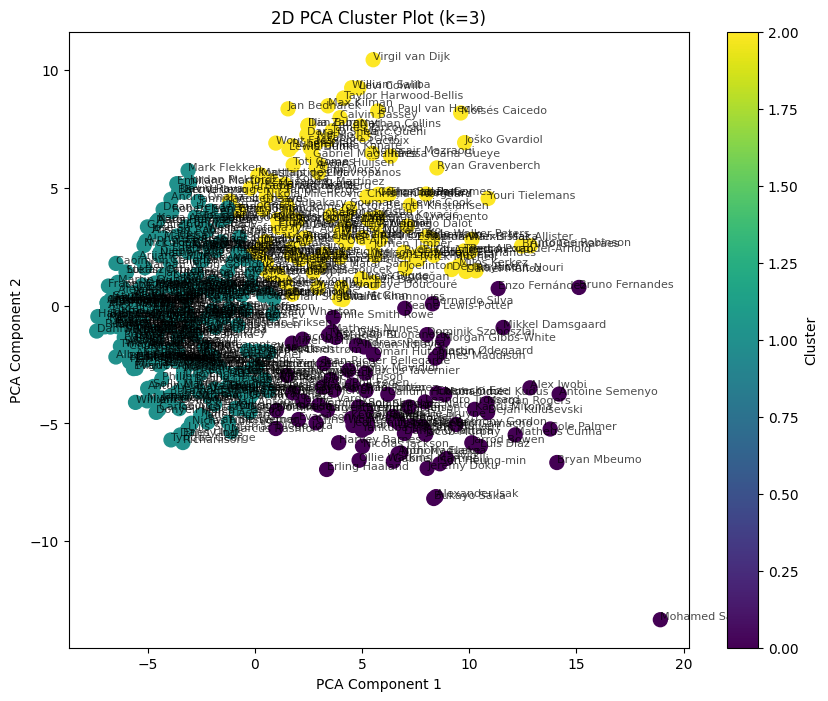
\includegraphics[width=1\textwidth]{clusters_2d.png}

\textbf{h) Conclusion} \\
The K-means clustering algorithm, combined with PCA for dimensionality reduction, provides an effective way to group football players based on their performance statistics. The 2D visualization of the clusters offers a clear representation of how players from different positions and playing styles are grouped. This methodology not only aids in understanding player roles but also provides a foundation for further analysis of player performance across different metrics.

The results can be used to identify patterns in player performance, highlight strengths and weaknesses within specific clusters, and inform strategies for team composition based on player characteristics.
\newpage
%_______Kết luận________
\section*{\textcolor{blue}{\Large 5. Player Value Estimation}}
\titleformat{\section}
  {\bfseries\Large}
  {\thesection.}{1em}{}
\subsection*{\textbf{5.1. Collect valuable player transfer data (2024-2025)}}
Initialize an Incognito Browser:
\begin{itemize}
    \item Use Selenium with Chrome in headless mode to increase speed and reduce resources.
    \item Configure a user-agent to simulate a real browser.
\end{itemize}
\begin{mdframed}
\begin{verbatim}
chrome_options = Options()
chrome_options.add_argument("--headless")
chrome_options.add_argument("--disable-gpu")
driver = webdriver.Chrome(options=chrome_options)
\end{verbatim}
\end{mdframed}
Open the website containing the player transfer value data.
Make sure the page loads completely before extracting the data.\\
Use Selenium's get() method to open the web page.
\begin{mdframed}
\begin{verbatim}
    driver.get(url)
\end{verbatim}
\end{mdframed}
The site uses JavaScript to load dynamic data → Need to wait enough time for all content to display.
\begin{mdframed}
\begin{verbatim}
    time.sleep(10)
\end{verbatim}
\end{mdframed}
Value 10 seconds: Ensures enough loading time, can be adjusted depending on network speed, enough for the site to fully render in most cases.
\setlist[itemize]{noitemsep, topsep=0pt}











\newpage
%_______Kết luận________
\section*{\textcolor{blue}{\Large 6. Conclusion}}
\titleformat{\section}
  {\bfseries\Large}
  {\thesection.}{1em}{}

\setlist[itemize]{noitemsep, topsep=0pt}

\textbf{a) Overview of K-means Clustering} \\
This project conducted a detailed analysis of football player performance data to evaluate team effectiveness, classify player roles, and forecast market values using machine learning techniques. The workflow included data preprocessing, K-means clustering, dimensionality reduction via PCA, and predictive modeling using Random Forest Regression. Visualization tools played a crucial role in making the findings more interpretable, ultimately providing deeper insights into the key factors that influence a player’s market worth.

\textbf{b) Overview of K-means Clustering} \\
Throughout the course of this project, we gained valuable practical experience in both data science and football analytics. Some of the major learning outcomes include:
\begin{itemize}
    \item Developing skills in gathering and extracting data from online platforms.
    \item Cleaning and standardizing real-world sports data for analytical use.
    \item Implementing clustering techniques to uncover natural player groupings based on performance metrics.
    \item Applying regression models to estimate outcomes such as player market value.
    \item 
    \item Drawing meaningful insights from statistical patterns within the football domain.
\end{itemize}

\textbf{c) Future Improvements} \\
While the current model has delivered promising results, there are several avenues for further improvement:
\begin{itemize}
    \item Expanding the dataset to include additional seasons, leagues, and a larger pool of players to enhance model reliability and applicability.
    \item Incorporating contextual variables such as injuries, playing time, or club financial data for a more comprehensive analysis.
    \item Exploring advanced regression models like XGBoost or deep learning approaches to boost prediction performance.
    \item Building an interactive dashboard that allows users to dynamically explore player statistics and clustering results.
\end{itemize}
In conclusion, this work lays a strong foundation for data-driven decision-making in contemporary football, supporting strategies related to talent scouting, performance assessment, and market evaluation.


\end{document}
